\begin{frame}
  \begin{center}
    {\Large Why do we need multiple layers?}
  \end{center}
\end{frame}

\begin{frame}
\begin{center}
  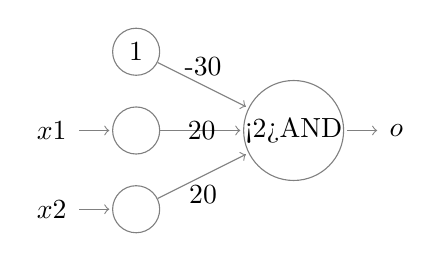
\begin{tikzpicture}[shorten >=1pt,->,draw=black!50, node distance=2.5cm]
    \tikzstyle{every pin edge}=[<-,shorten <=1pt]
    \tikzstyle{neuron}=[circle,draw,minimum size=17pt,inner sep=0pt]

    \node[neuron] (I-0) at (0,0) {$1$};
    \foreach \y in {1,2}
    \node[neuron, pin=left:$x\y$] (I-\y) at (0,-\y) {};

    \node[neuron,pin={[pin edge={->}]right:$o$}] (O-1) at
    (2.0,-1) {\only<2>{AND}};

    \path (I-0) edge node[above] {-30} (O-1);
    \path (I-1) edge node {20} (O-1);
    \path (I-2) edge node[below] {20} (O-1);
  \end{tikzpicture}
  \end{center}
\end{frame}

\begin{frame}
  \begin{center}
    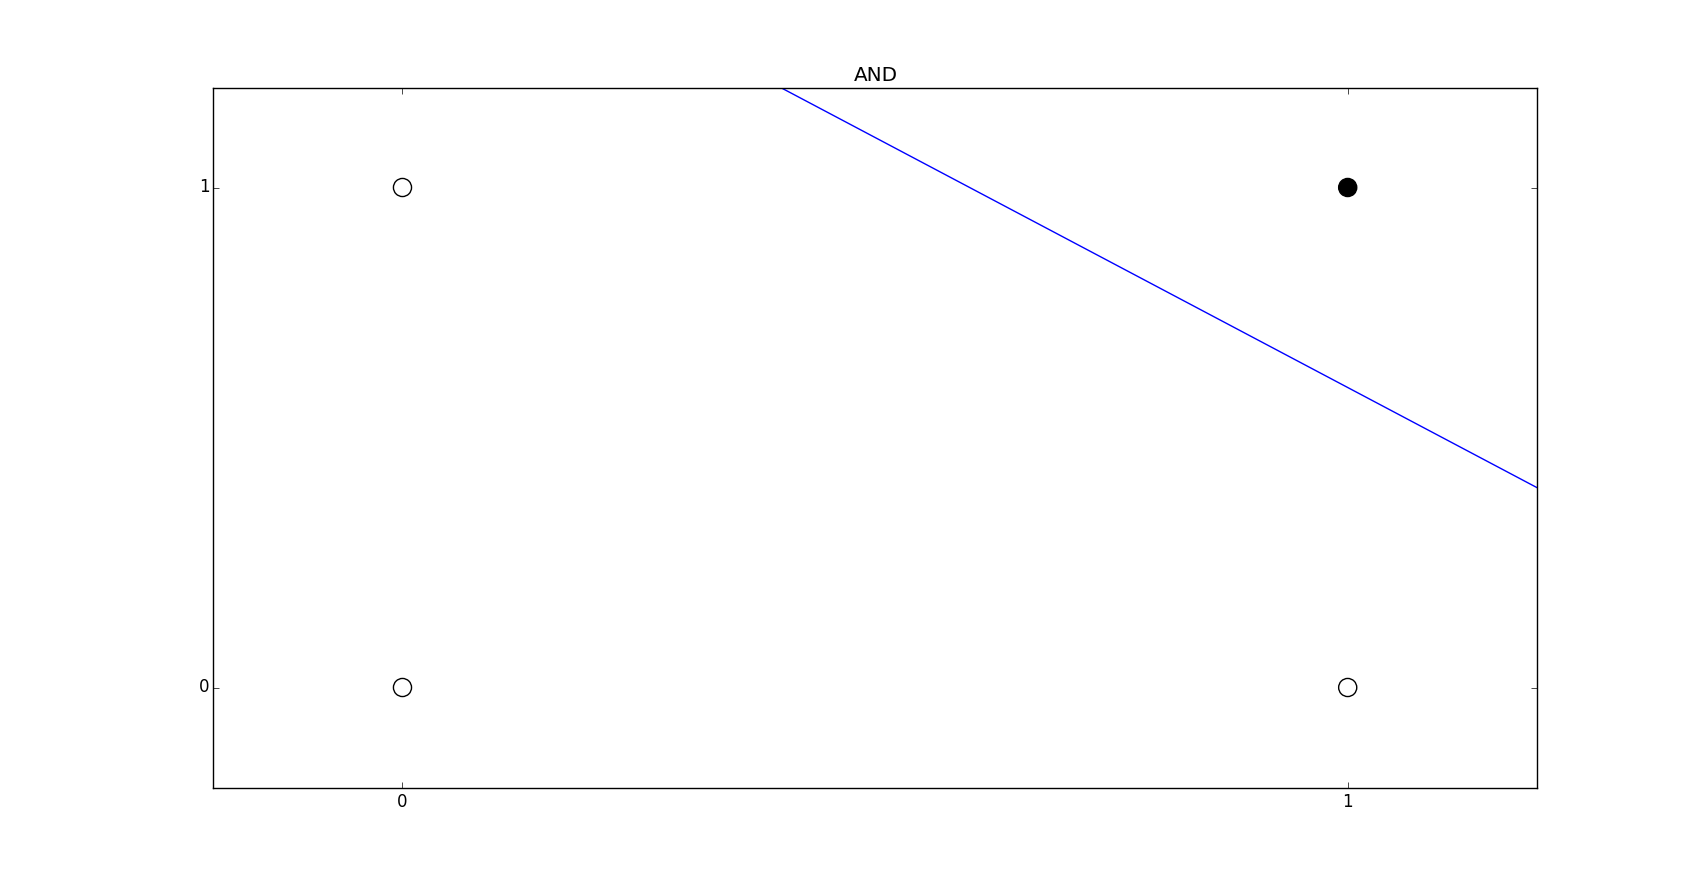
\includegraphics[scale=0.25]{pictures/and.png}
  \end{center}
\end{frame}

\begin{frame}
\begin{center}
  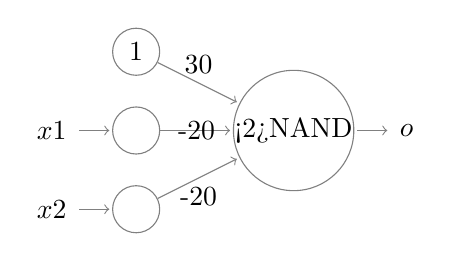
\begin{tikzpicture}[shorten >=1pt,->,draw=black!50, node distance=2.5cm]
    \tikzstyle{every pin edge}=[<-,shorten <=1pt]
    \tikzstyle{neuron}=[circle,draw,minimum size=17pt,inner sep=0pt]

    \node[neuron] (I-0) at (0,0) {$1$};
    \foreach \y in {1,2}
    \node[neuron, pin=left:$x\y$] (I-\y) at (0,-\y) {};

    \node[neuron,pin={[pin edge={->}]right:$o$}] (O-1) at
    (2.0,-1) {\only<2>{NAND}};

    \path (I-0) edge node[above] {30} (O-1);
    \path (I-1) edge node {-20} (O-1);
    \path (I-2) edge node[below] {-20} (O-1);
  \end{tikzpicture}
  \end{center}
\end{frame}

\begin{frame}
  \begin{center}
    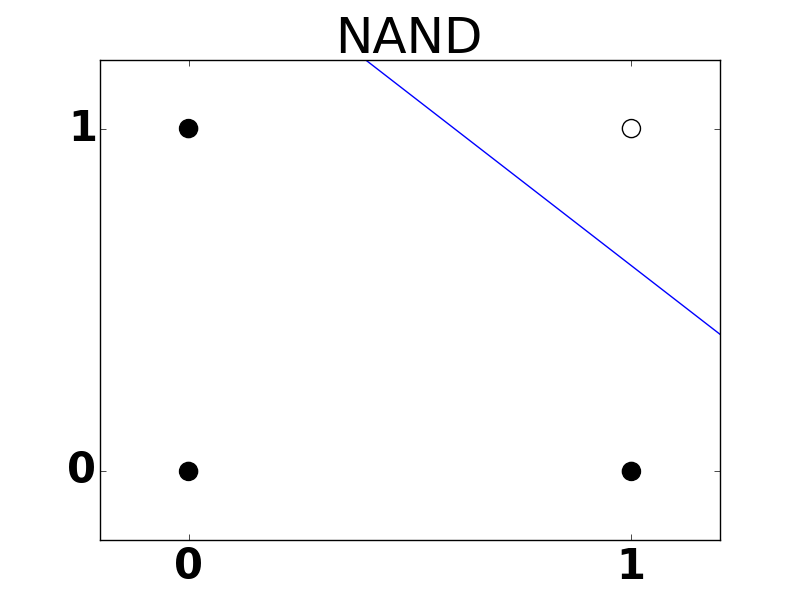
\includegraphics[scale=0.25]{pictures/nand.png}
  \end{center}
\end{frame}

\begin{frame}
\begin{center}
  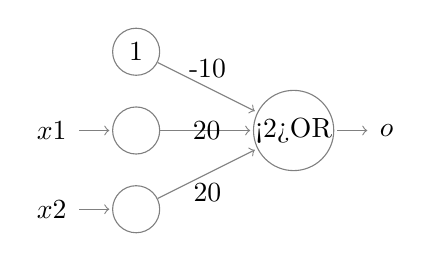
\begin{tikzpicture}[shorten >=1pt,->,draw=black!50, node distance=2.5cm]
    \tikzstyle{every pin edge}=[<-,shorten <=1pt]
    \tikzstyle{neuron}=[circle,draw,minimum size=17pt,inner sep=0pt]

    \node[neuron] (I-0) at (0,0) {$1$};
    \foreach \y in {1,2}
    \node[neuron, pin=left:$x\y$] (I-\y) at (0,-\y) {};

    \node[neuron,pin={[pin edge={->}]right:$o$}] (O-1) at
    (2.0,-1) {\only<2>{OR}};

    \path (I-0) edge node[above] {-10} (O-1);
    \path (I-1) edge node {20} (O-1);
    \path (I-2) edge node[below] {20} (O-1);
  \end{tikzpicture}
  \end{center}
\end{frame}

\begin{frame}
  \begin{center}
    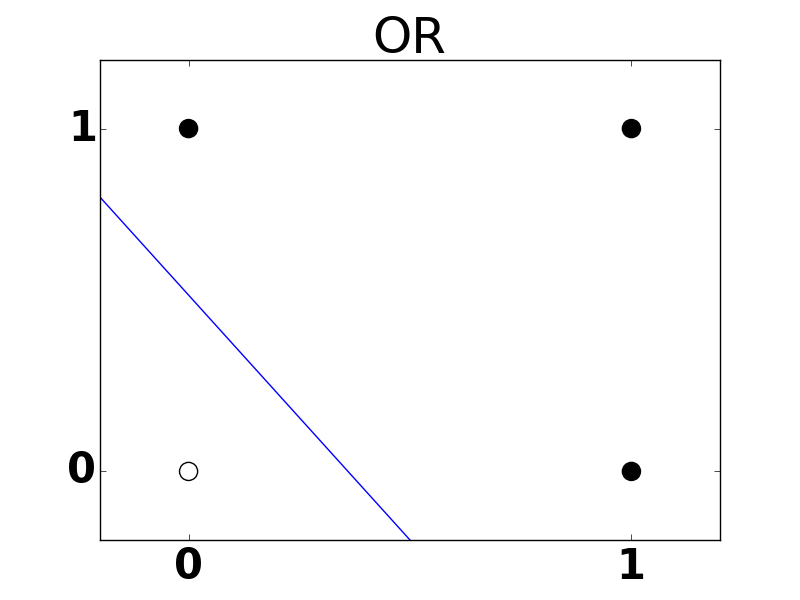
\includegraphics[scale=0.25]{pictures/or.png}
  \end{center}
\end{frame}

\begin{frame}
  \begin{center}
    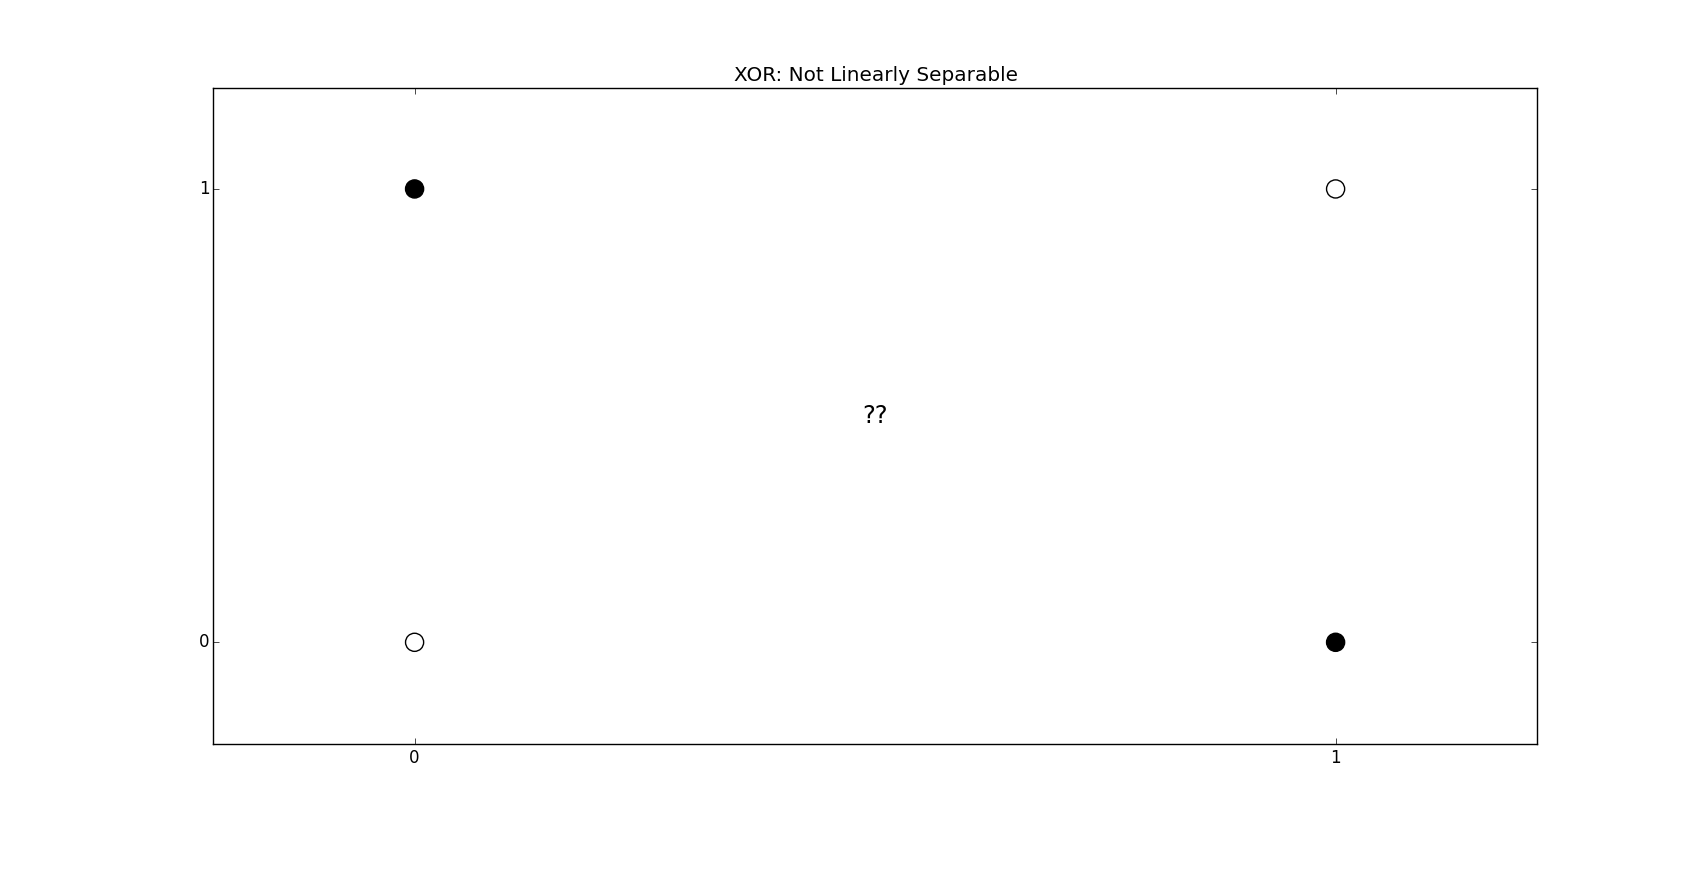
\includegraphics[scale=0.25]{pictures/xor.png}
  \end{center}
\end{frame}

\begin{frame}
\begin{center}
\frametitle{XOR}
  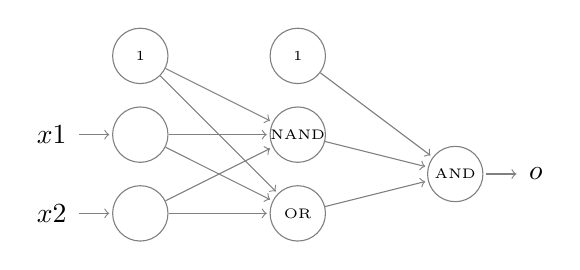
\begin{tikzpicture}[shorten >=1pt,->,draw=black!50, node distance=2.5cm]
    \tikzstyle{every pin edge}=[<-,shorten <=1pt]
    \tikzstyle{neuron}=[circle,draw,minimum size=20pt,inner sep=0pt,font=\tiny]

    \node[neuron] (I-0) at (0,0) {$1$};
    \foreach \y in {1,2}
    \node[neuron, pin=left:$x\y$] (I-\y) at (0,-\y) {};

    \node[neuron] (H-0) at (2.0,0) {1};
    \node[neuron] (H-1) at (2.0,-1) {NAND};
    \node[neuron] (H-2) at (2.0,-2) {OR};

    \node[neuron,pin={[pin edge={->}]right:$o$}] (O-1) at (4,-1.5) {AND};

    \path (I-0) edge (H-1);
    \path (I-1) edge (H-1);
    \path (I-2) edge (H-1);
    \path (I-0) edge (H-2);
    \path (I-1) edge (H-2);
    \path (I-2) edge (H-2);

    \path (H-0) edge (O-1);
    \path (H-1) edge (O-1);
    \path (H-2) edge (O-1);
  \end{tikzpicture}
  \end{center}
\end{frame}

\begin{frame}{Forward propagation}
\SetKwProg{Fn}{}{}{end}\SetKwFunction{ForwardProp}{ForwardPropagation}
\begin{algorithm}[H]
\Fn(){\ForwardProp{x, w}}{
$o^1 \gets x$\;
\For{l = 2 to L}{
$x = add\_bias(o^{l-1})$\;
$o^l = g((w^l)^T x)$\;
}
$return~o$\;
}
\end{algorithm}
\end{frame}

\begin{frame}
  \begin{center}
    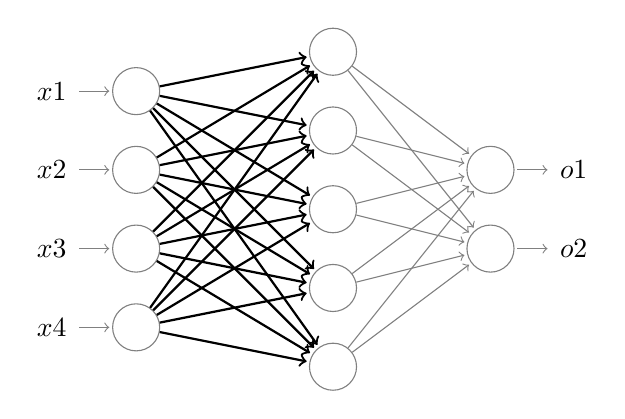
\begin{tikzpicture}[shorten >=1pt,->,draw=black!50, node distance=2.5cm]
      \tikzstyle{every pin edge}=[<-,shorten <=1pt]
      \tikzstyle{neuron}=[circle,draw,minimum size=17pt,inner sep=0pt]

      % input layer nodes
      \foreach \y in {1,...,4}
      \node[neuron, pin=left:$x\y$] (I-\y) at (0,-\y) {};

      % hidden layer nodes
      \foreach \y in {1,...,5}
      \path[yshift=0.5cm]
      node[neuron] (H-\y) at (2.5,-\y) {};

      % output layer node
      \foreach \y in {1,2}
      \path[yshift=-1cm]
      node[neuron,pin={[pin edge={->}]right:$o\y$}] (O-\y) at (4.5,-\y) {};

      % Connect every node in the input layer with every node in the
      % hidden layer.
      \foreach \src in {1,...,4}
      \foreach \dst in {1,...,5}
      \path[draw=black,thick] (I-\src) edge (H-\dst);

      % Connect every node in the hidden layer with the output layer
      \foreach \src in {1,...,5}
      \foreach \dst in {1,2}
      \path (H-\src) edge (O-\dst);
    \end{tikzpicture}
  \end{center}
\end{frame}

\begin{frame}
  \begin{center}
    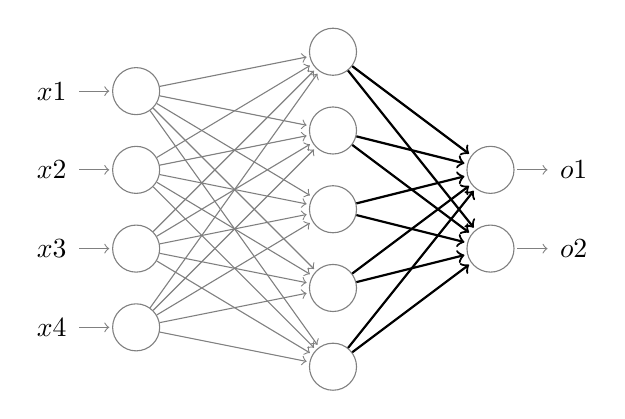
\begin{tikzpicture}[shorten >=1pt,->,draw=black!50, node distance=2.5cm]
      \tikzstyle{every pin edge}=[<-,shorten <=1pt]
      \tikzstyle{neuron}=[circle,draw,minimum size=17pt,inner sep=0pt]

      % input layer nodes
      \foreach \y in {1,...,4}
      \node[neuron, pin=left:$x\y$] (I-\y) at (0,-\y) {};

      % hidden layer nodes
      \foreach \y in {1,...,5}
      \path[yshift=0.5cm]
      node[neuron] (H-\y) at (2.5,-\y) {};

      % output layer node
      \foreach \y in {1,2}
      \path[yshift=-1cm]
      node[neuron,pin={[pin edge={->}]right:$o\y$}] (O-\y) at (4.5,-\y) {};

      % Connect every node in the input layer with every node in the
      % hidden layer.
      \foreach \src in {1,...,4}
      \foreach \dst in {1,...,5}
      \path (I-\src) edge (H-\dst);

      % Connect every node in the hidden layer with the output layer
      \foreach \src in {1,...,5}
      \foreach \dst in {1,2}
      \path[draw=black,thick] (H-\src) edge (O-\dst);
    \end{tikzpicture}
  \end{center}
\end{frame}
